%
%
%
%
\section{Introduction}\label{sec:intro}
A point set $P\subset[0,1)^s$ of $N$ points is \emph{quasi-uniform} if its covering radius $h(P)$, the radius of the largest empty ball, and its separation $\delta(P)$, the smallest distance between two of its points, are both of the optimal order $N^{-1/s}$; equivalently, the mesh ratio $h(P)/\delta(P)$ is bounded. For a sequence the condition is asked of every prefix $P_{[N]}$, the first $N$ points, for all $N$ at once. Dick, Goda and Suzuki \cite{DGS2}, continuing Part~I with Larcher and Pillichshammer \cite{DGLPS1}, asked for digital nets and sequences in a fixed base that are both low-discrepancy and quasi-uniform. Their positive example is the two-dimensional Larcher--Pillichshammer net \cite{LP01}; for dimension $s\ge3$ they state the construction as open, for nets and for sequences, and Suzuki \cite{Suz26} recently wrote that no such family is known there. Goda, Hofer and Suzuki proved that the Halton sequences are not quasi-uniform and asked whether any Halton-type sequence is \cite[Open Problem~2]{GHS26}. The companion paper \cite{Gru26geo}%
\ answers the question of Dick, Goda and Suzuki for nets in every dimension. This paper answers it for sequences, and settles the question of Goda, Hofer and Suzuki: no Halton-type sequence is quasi-uniform.

\emph{The classical sequences fail.} The Halton, Faure, Sobol' and Niederreiter sequences are built from polynomial bases: each coordinate reads the index, written as a polynomial over a finite field, in its own base, one block of digits at a time. Their prefixes of $q^m$ points are nets at every scale, so their covering radius is always of the right order. Their separation is not, and the reason is a carry (Figure~\ref{fig:carry}). Take two indices whose difference is a carry in the last digits of one coordinate: in base $p$ the digits $0.a(p-1)\cdots(p-1)$ of one point become $0.(a+1)0\cdots0$ for the other, and the two points sit on either side of a cell boundary. If the same difference is divisible by a high power of every other base, it leaves the leading digits of all other coordinates unchanged, and the two points are close in every coordinate at once. For polynomial bases such differences exist at infinitely many sizes. In the carrying base $b$ a carry is a run of ones, $1+b+\dots+b^{\nu-1}=(b^\nu-1)/(b-1)$, and this run is divisible by all the other bases as soon as $b^\nu\equiv1$ modulo $b-1$ times their product, which holds for suitable $\nu$. The Frobenius map $f\mapsto f^p$, which is additive in characteristic $p$, then stretches one such pair into a pair at $p$ times the scale, and the excess of the shared digits over the cell side grows each time. Theorem~\ref{thm:nonqu} turns this into explicit close pairs for every digital sequence whose coordinates read the index in pairwise coprime polynomial bases, one of them as a radical inverse.

Table~\ref{tab:negative} lists the consequences. In dimension $s\ge2$ no Halton-type sequence is quasi-uniform, which answers Open Problem~2 of \cite{GHS26} with explicit index pairs (Corollary~\ref{cor:halton}); neither is any Faure sequence (Corollary~\ref{cor:faure}), any Sobol' sequence (Corollary~\ref{cor:sobol}) or any classical Niederreiter sequence (Corollary~\ref{cor:nied}); and scrambling every coordinate but one does not help (Corollary~\ref{cor:unscrambled}). These statements were not found in the literature we searched (through October 2026); the earlier results are listed in the table. So, among sequences of this kind, a quasi-uniform one has to scramble every coordinate beyond a scalar, and the natural repair is a scramble that lets the coordinates see each other's carries.

\begin{table}[t]
\centering
\small
\caption{Classical sequences that are not quasi-uniform (Section~\ref{sec:fail}). All are digital sequences in dimension $s\ge2$; every result gives explicit close pairs along an explicit sequence of sizes (Theorem~\ref{thm:nonqu}). ``Earlier'': the cases known before, as far as we found.}
\label{tab:negative}
\setlength{\tabcolsep}{3pt}
\begin{tabular}{@{}>{\raggedright\arraybackslash}p{0.17\textwidth}>{\raggedright\arraybackslash}p{0.39\textwidth}>{\raggedright\arraybackslash}p{0.25\textwidth}>{\raggedright\arraybackslash}p{0.13\textwidth}@{}}
\toprule
sequences & scope & earlier & where\\
\midrule
polynomial-base digital sequences & pairwise coprime bases $b_c\in\F_q[z]$ of any degrees, every coordinate $b_c$-adic, one coordinate a radical inverse & -- & Thm.~\ref{thm:nonqu}\\
Halton-type & every prime $p$, every $s\ge2$, any pairwise coprime bases in $\F_p[z]$, monic or not, irreducible or not \cite[Def.~2]{GHS26} & Halton sequences and three families of Halton-type sequences \cite{GHS26} & Cor.~\ref{cor:halton}\\
Faure, unscrambled frames & $(\Pas^0,\dots,\Pas^{s-1})$ in prime base $p$, every $2\le s\le p$; any distinct places over $\F_q$; separation at most of order $N^{-1/(s-1)}$ along a sequence of $N$ when two places differ by $1$ & $s=p$ \cite{DGS2}; $s=2$ and $s=p$ \cite{GHS26} & Cor.~\ref{cor:faure}, Rem.~\ref{rem:faurerate}\\
Sobol' & every $s\ge2$, any admissible direction numbers, with or without the van der Corput coordinate, natural or Gray-code order, every projection to $s'\ge2$ coordinates & $s=2$ \cite{Goda23,Suz25}; the opposite was suggested numerically \cite{SS07} & Cor.~\ref{cor:sobol}\\
Niederreiter & classical, over every $\F_q$ (natural identification); generalized, when one coordinate is a radical inverse & -- & Cor.~\ref{cor:nied}\\
one coordinate unscrambled & bases as in Thm.~\ref{thm:nonqu}; one coordinate a radical inverse up to a scalar, all others with any fixed lower-triangular scramble; for a linear base also a diagonal scramble & Faure, $s=p$ (every prime $p$), first coordinate unscrambled \cite[Rem.~3]{GHS26}; $(L,\Pas)$, $(I,L\Pas)$ in base $2$ \cite[Thm.~4.2]{DGS2} & Cor.~\ref{cor:unscrambled}\\
randomizations & digital shifts, Faure--Tezuka index scrambles, reorderings that keep every full level as a set; a fixed Toeplitz scramble of the carrying coordinate with rational multiplier (under a squarefree condition) & Owen scrambling: almost surely not quasi-uniform \cite{Suz26} & Rem.~\ref{rem:randomize}, \ref{rem:toeplitz}\\
\bottomrule
\end{tabular}
\end{table}

\emph{Why sequences are harder than nets.} The nets of \cite{Gru26geo} also scramble the generalized Faure sequences, but anew for every number of points. At a full level $N=q^{sK}$ the prefix of a $(0,s)$-sequence has exactly one point in each cell of side $N^{-1/s}$, so what decides the separation is where each point sits inside its cell relative to its neighbours. To first order this position is given by the \emph{geometric digits}, the first digit of each coordinate below the cell. They are a linear function of the cell digits, the \emph{offset map}. What matters for the separation are its \emph{carry responses}: how the geometric digits change when one cell index steps to the next cell, across a boundary where $l$ of its digits change (a carry of length $l$). For the Faure sequence the offset map changes with the level: in dimension two one of its coefficients is $(-1)^K(K+1)$ at level $K$, which runs through all residues modulo $p$ (Example~\ref{ex:faurelaw}). A net can undo this with a scramble chosen for its size. A sequence cannot: a row of its scramble, once used, stays in use at every finer level, so one fixed scramble has to serve all scales. The natural candidates are the \emph{self-similar} scrambles. Let $a_c$ be the point at which coordinate $c$ reads the index (its \emph{place}). Multiplying the index polynomial by $w=\prod_c(z-a_c)$ takes the cell picture one level finer, and for a self-similar scramble it shifts the digits of every coordinate by one place and multiplies them by one fixed scale. Such scrambles have the same offset map at every level (Proposition~\ref{prop:law}), and then one finite check bounds the separation at every level (Lemma~\ref{lem:cert}). What remains is to choose the infinitely many carry responses, one for each carry length, all of them well. How much of this exact linear rules of bounded depth can do is limited (Theorem~\ref{thm:count} below).

\emph{The fix: residues.} A Taylor coefficient of the index polynomial $V$ at a point $a$ is a residue, $[(z-a)^n]V=\Res_a\bigl(V(z-a)^{-n-1}dz\bigr)$. More generally, every scramble of a generalized Faure sequence reads digit $n$ of coordinate $c$ as the residue at the place $a_c$ of $V$ times a differential with a pole of order $n+1$ there (Lemma~\ref{lem:resform}). The residues of one rational function at all its poles on the projective line add up to zero. So if all coordinates read their digits from one rational differential, the residue theorem is a linear identity between digits of different coordinates. It holds at every level and involves no carries: a carry in one coordinate is now seen by the others. In the simplest example, the \emph{brick wall} in dimension two, the identity says that the height of a point inside its cell in coordinate~$1$ is half the finest cell digit of coordinate~$0$, at every level: neighbouring columns of points are staggered by half a cell, like the courses of a brick wall (Section~\ref{sec:law}).

This gives two closed forms (Section~\ref{sec:residue}). In the \emph{staggered residue sequence}, the brick wall in every dimension, one coordinate is staggered by a rank-1 lattice rule in the cell indices of the others; it is certified at every full level for every prime $p>2^s$, with the constant $(\lfloor p/2^{s-1}\rfloor-1)/p$, which is the best this one-coordinate bound allows (Corollary~\ref{cor:dyadic}). The \emph{residue sequence} lets every coordinate read the same differential $V\,dz$. The residue theorem then relates the last cell digits of all coordinates at the prefixes $P_{sK-1}$, one digit before each full level. Give one coordinate one cell digit fewer than the others, so that every box of these depths holds one point (a \emph{skeleton coordinate} in the language of \cite{Gru26geo}): its next digit is then a fixed linear combination of the finest cell digits of the other coordinates, the \emph{skeleton relation}. As a result the points of $P_{sK-1}$ occupy exactly those \emph{fine cells}, the cubes of side $p^{-K}$, whose indices lie in the Construction-A lattice $\Lambda_v=\{b\in\Z^s:\sum_cv_cb_c\equiv0\pmod p\}$ of a \emph{check vector} $v\in(\F_p^*)^s$, one point in each (Theorem~\ref{thm:residue}, Figure~\ref{fig:residue}). This is the picture of the nets of \cite{Gru26geo}: a lattice image plus a jitter of less than one fine cell%
, now produced at every $m\equiv-1\pmod s$ by one fixed scramble. With a Korobov check vector the separation there is at least $(\rho-1)p^{-1/s}>1-2p^{-1/s}$, $\rho=\lfloor p^{1/s}\rfloor$, in every dimension (Corollary~\ref{cor:korobov}); with searched check vectors it exceeds $1$, the value of the cubic grid, already at moderate primes, because the lattice $\Lambda_v$ can be close to a denser packing than the grid (the hexagonal lattice has $1.0746$ in the plane).

The nets of \cite{Gru26geo} go further at the full levels: they prescribe all $s$ geometric digits by a fixed linear rule in the last few cell digits, a \emph{design}, and this is how they reach separations $1-O(1/q)$. A scramble puts one factor in front of the differential at each place, its \emph{local multiplier}. Reading the digits in blocks of $s$, with $s$ different local multipliers per coordinate, the residue theorem installs such a design%
\ at every $s$-th full level: the \emph{block-periodic residue sequences} have separation $1-2/p$ at $N=p^{4K}$ in dimension two and at $N=p^{9K}$ in dimension three, for every prime $p\ge3$ resp.\ $p\ge5$, with a short proof (Theorem~\ref{thm:block}).

\emph{Level families.} Each construction is certified at its own family of sizes $N=p^m$, its \emph{level family} (Figure~\ref{fig:levels}): $m\equiv-1$ or $m\equiv0\pmod s$, or $m\in s^2\N$. Every family with bounded gaps gives a bound for all $N$ (Lemma~\ref{lem:prefix}), and hence quasi-uniformity, but the bound loses the factor $p^{-\Delta/s}$, where $\Delta$ is the largest gap. So a denser family can win for all $N$ even with a smaller constant at its certified sizes: the residue sequences give $\LB/p$ for all $N$, the block-periodic sequences only $\LB/p^s$.

\begin{figure}[t]
\centering
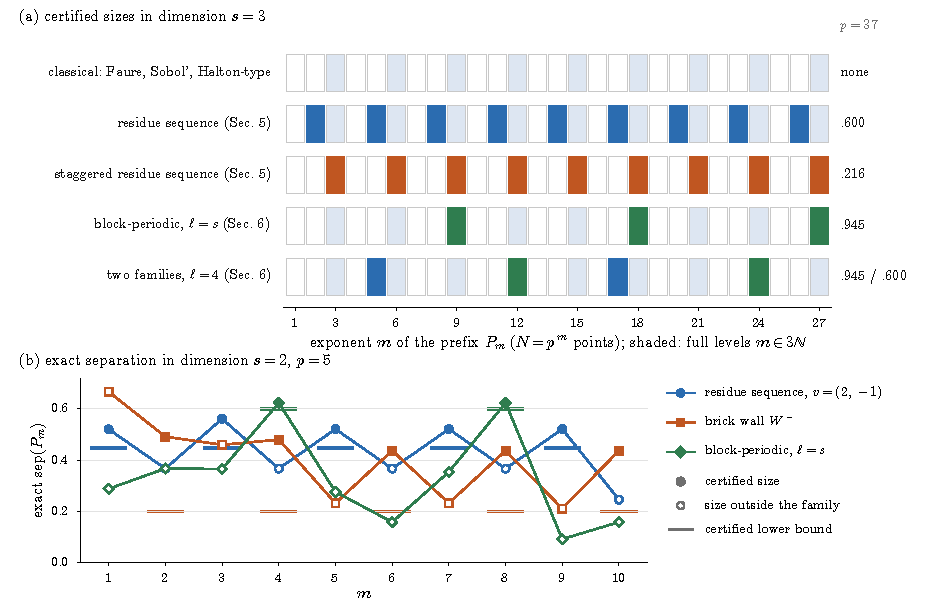
\includegraphics[width=0.9\linewidth]{fig_levels.pdf}
\caption{Level families. (a)~The exponents $m\le27$ at which each construction has a certified lower bound on $\sep{P_m}$ in dimension $s=3$ (filled; shaded columns are the full levels), with the certified constant at $p=37$: residue sequence, best check vector of Table~\ref{tab:residue} (Theorem~\ref{thm:residue}); staggered residue sequence with dyadic weights, $8/37$ (Corollary~\ref{cor:dyadic}); block-periodic residue sequence, $1-2/37$ (Theorem~\ref{thm:block}(b)); block period $\ell=4$ (Theorem~\ref{thm:blocktwo}): the design at $m\in12\N$ and skeleton relations at $m=5,17,29,\dots$ (blue). The classical sequences have no certified level; they fail along explicit sequences of levels (Section~\ref{sec:fail}). (b)~Exact $\sep{P_m}$, $m=1,\dots,10$, in dimension two over $\F_5$: the residue sequence with the Korobov vector $v=(2,-1)$ (certified $0.447$ at odd $m$), the brick wall $W^-$ (certified $0.2$ at even $m$, Theorem~\ref{thm:WF}) and the block-periodic sequence of Theorem~\ref{thm:block}(a) (certified $0.6$ at $m\in4\N$). Filled markers: sizes in the level family; bars: the certified bounds. Off its family a sequence is not controlled: the block-periodic sequence falls to $0.092$ at $m=9$ and the residue sequence to $0.246$ at $m=10$. Exact computations from the generator matrices.}
\label{fig:levels}
\end{figure}

\emph{What more is possible, and what is not.} Why not $s$ exact relations at every full level, which would put the design of the nets into every full level of one sequence? Within the scrambles of generalized Faure sequences, and for exact linear relations of bounded depth among the digits, this is impossible: a late enough range of $R+1$ consecutive levels carries at most $J+R+1$ independent relations of depth at most $J$, about one per level (Theorem~\ref{thm:count}, a residue-theorem argument at a single place). So all $s$ geometric digits can be designed on at most a fraction $1/s$ of the full levels, which the block-periodic sequences attain (Corollary~\ref{cor:layer}); the skeleton relations of the residue sequence and designed geometric digits share one count (Corollary~\ref{cor:density}); and no designed geometric digit fits at a full level next to skeleton relations (Corollary~\ref{cor:nodesign}). Section~\ref{sec:count} states the scope of each of these statements. To reach every full level with constants tending to $1$, Section~\ref{sec:antipode} uses certificates that are not exact relations: it keeps each carry response inside a fixed set of allowed values, a \emph{window}, by choosing the free digits of a self-similar scramble one at a time. Half a cell is, up to $1/p$, the only offset that is equally good for a forward step, a backward step and no step (Lemma~\ref{lem:antipode}); staggering one coordinate by half a cell against all the others gives $1-O(1/p)$ at every full level for large primes, in every dimension (Theorem~\ref{thm:A}). In a stated scope, windows and the skeleton relations of the residue sequence cannot be selected together (Proposition~\ref{prop:joint}).

\emph{Results.} All sequences of this paper are explicit linear scrambles of generalized Faure sequences, hence digital $(0,s)$-sequences, with star discrepancy $O((\log N)^s/N)$ \cite{Nie92}. Each comes with a lower bound on $\sep{P_m}=\delta(P_m)N^{1/s}$ at every $m$ of its level family and is therefore quasi-uniform. Table~\ref{tab:results} lists the results; the headlines are these.
\begin{enumerate}
\item \emph{The classical sequences fail} (Section~\ref{sec:fail}, Table~\ref{tab:negative}), with explicit close pairs.
\item \emph{A closed form in every dimension.} For every $s\ge2$ and every prime $p>2^s$ the residue sequence with a Korobov check vector is a quasi-uniform digital $(0,s)$-sequence with $\sep{P_{sK-1}}\ge(\rho-1)p^{-1/s}>1-2p^{-1/s}$ for every $K$ (Theorem~\ref{thm:residue}, Corollaries~\ref{cor:korobov} and~\ref{cor:residueQU}), and the staggered residue sequence has $\sep{P_{sK}}\ge(\lfloor p/2^{s-1}\rfloor-1)/p$ for every $K$ (Corollary~\ref{cor:dyadic}). With searched check vectors the constant of the residue sequence reaches $1.024$ in dimension two ($p=1009$) and $1.035$ in dimension three ($p=10007$) (Table~\ref{tab:residue}).
\item \emph{Separation $1-O(1/p)$ from small primes on, at every $s$-th full level.} The block-periodic residue sequences have $\sep{P_{s^2K}}\ge1-2/p$ for every prime $p\ge3$ ($s=2$) and $p\ge5$ ($s=3$), and $1-(a^*_s+1)/p$ in every dimension $s\ge4$ for $p\ge5a^*_s+4$; with a smaller diagonal of the design, $1-4/p$, $1-8/p$, $1-15/p$, $1-60/p$ for $s=4,\dots,7$ and every prime $p\ge11$, $23$, $37$, $191$ (Theorem~\ref{thm:block}; computer-assisted for these four).
\item \emph{Limits of exact relations} (Section~\ref{sec:count}): about one exact relation of bounded depth per level, in the scope stated there.
\item \emph{Every full level.} For every $s\ge3$ a closed form gives $\sep{P_{sK}}\ge1-C''_s/p$ for every prime $p\ge p_0(s)$ (Theorem~\ref{thm:A}), in dimension three $1-742/p$ for every prime $p\ge1.97\cdot10^7$ (Theorem~\ref{thm:A3}); in dimension two, $1-17/p$ for every prime $p>3677$ (Corollary~\ref{cor:HB17}).
\item \emph{Every base in small dimensions} (Theorem~\ref{thm:coverage}, which lists the level families). In dimension two every prime base is covered (base $3$ by Theorem~\ref{thm:block}(a) and, at every full level, by a computer-assisted bound); in base $2$ the sequence is a two-sided scramble of the Sobol' sequence with $\sep{P_{2K}}\ge0.3678$, which answers a question of Dick, Goda and Suzuki \cite[Section~4.2]{DGS2}: it is well-separated in their sense \cite[Def.~3.8]{DGS2} (Theorem~\ref{thm:B2}). In dimension three every prime base $p\ge3$ is covered, base $5$ at the sizes $5^{9K}$ only, and base $4$; in dimension four every prime $p\ge7$ and base $4$; in dimension five every prime $p\ge11$; in dimension six every prime $p\ge17$; in every dimension $s$ every prime $p>2^s$; and prime-power bases in dimensions two to five (Table~\ref{tab:primepower}).
\end{enumerate}

\begin{table}[t]
\centering
\footnotesize
\setlength{\tabcolsep}{2.3pt}
\caption{The main results: digital $(0,s)$-sequences in base $q$ with $\sep{P_m}\ge\LB$, the entry of the fourth column, for every $m$ in the stated level family, hence quasi-uniform; the fifth column is the resulting bound $\delta(P_{[N]})N^{1/s}\ge\cdot$ for every $N\ge2$ (Lemma~\ref{lem:prefix}). Form: \emph{closed}, explicit functions of $p$ (for the window constructions with any admissible choice of the free digits); \emph{table}, a finite certificate. Proof: \emph{proof${}^\star$}, the last step is one exact rational evaluation; \emph{c.a.}, computer-assisted (Section~\ref{sec:conventions}). $\rho=\lfloor p^{1/s}\rfloor$; $a^*_4=5$, $a^*_5=16$. First row: the closed form $(\rho-1)p^{-1/s}$ is proved; the values for searched check vectors $v$ are exact finite evaluations (c.a.). Not listed: the sequences of Theorem~\ref{thm:blocktwo} and Corollary~\ref{cor:gauss}, which are certified on two level families at once.}
\label{tab:results}
\begin{tabular}{@{}c>{\raggedright\arraybackslash}p{0.15\textwidth}l>{\raggedright\arraybackslash}p{0.25\textwidth}lll>{\raggedright\arraybackslash}p{0.13\textwidth}@{}}
\toprule
$s$ & base & levels $m$ & $\sep{P_m}\ge$ & all $N$ & form & proof & where\\
\midrule
$\ge2$ & prime $p>2^s$ & $s\N-1$ & $(\rho-1)p^{-1/s}>1-2p^{-1/s}$; searched $v$: $1.024$ ($s=2$), $1.035$ ($s=3$) & $\LB/p$ & closed & proof; c.a. & Thm.~\ref{thm:residue}, Cor.~\ref{cor:korobov}, Tab.~\ref{tab:residue}\\
$\ge2$ & prime $p>2^s$ & $s\N$ & $(\lfloor p/2^{s-1}\rfloor-1)/p$ & $\LB/p$ & closed & proof & Cor.~\ref{cor:dyadic}\\
$2$ & prime $p\ge3$ & $4\N$ & $1-2/p$ & $\LB/p^2$ & closed & proof & Thm.~\ref{thm:block}\\
$3$ & prime $p\ge5$ & $9\N$ & $1-2/p$ & $\LB/p^3$ & closed & proof & Thm.~\ref{thm:block}\\
$4$; $5$ & prime $p\ge11$; $23$ & $16\N$; $25\N$ & $1-4/p$; $1-8/p$ & $\LB/p^s$ & closed & c.a. & Thm.~\ref{thm:block}\\
$6$; $7$ & prime $p\ge37$; $191$ & $36\N$; $49\N$ & $1-15/p$; $1-60/p$ & $\LB/p^s$ & closed & c.a. & Thm.~\ref{thm:block}\\
$\ge4$ & prime $p\ge5a^*_s+4$ & $s^2\N$ & $1-(a^*_s+1)/p$ & $\LB/p^s$ & closed & proof & Thm.~\ref{thm:block}\\
$\ge3$ & prime $p\ge p_0(s)$ & $s\N$ & $1-C''_s/p$ & $\LB/p$ & closed & proof & Thm.~\ref{thm:A}\\
$3$ & prime $p\ge1.97\cdot10^7$ & $3\N$ & $1-742/p$ & $\LB/p$ & closed & proof${}^\star$ & Thm.~\ref{thm:A3}\\
$2$ & prime $p>3677$ & $2\N$ & $1-17/p$ & $\LB/p$ & closed & proof${}+{}$c.a. & Cor.~\ref{cor:HB17}\\
$2$ & $2$ & $2\N$ & $0.3678$ & $\LB/2$ & closed & c.a. & Thm.~\ref{thm:B2}\\
$3$ & $3$; $4$ & $3\N$ & $0.05598$; $0.11293$ & $\LB/q$ & closed & c.a. & Thms.~\ref{thm:S3}, \ref{thm:K4}\\
$3$ & $7$ & $3\N$ & $1/7$ & $\LB/7$ & table & c.a. & Thm.~\ref{thm:p7}\\
$4$ & $4$ & $4\N$ & $0.03013$ & $\LB/4$ & closed & c.a. & Thm.~\ref{thm:S4}\\
$2$--$5$ & $\F_8,\dots,\F_{169}$ (Tab.~\ref{tab:primepower}) & $s\N$ & Table~\ref{tab:primepower} & $\LB/q$ & closed & c.a. & Prop.~\ref{prop:primepower}\\
\bottomrule
\end{tabular}
\end{table}

\emph{Small bases and practice.} In the bases $2$, $3$ and $4$ neither residues nor windows give anything at every full level. There we choose frames whose local roots are lacunary series, such as $\sum_kx^{2^k}$, so that the responses are computed by a small finite automaton and the bound at every level is one finite minimum (Section~\ref{sec:frames}). Section~\ref{sec:frames} also reads the staggered residue sequence over prime-power fields and collects the coverage by dimension. In practice (Section~\ref{sec:practice}) the residue sequences are generated like any digital sequence, from closed-form matrices, and they stay certified under digital shifts (Lemma~\ref{lem:shift}). In dimension three their smallest $\sep{P_{[N]}}$ over $64\le N\le2^{23}$ is $0.235$ to $0.267$ at $p=13$, $17$, $23$, $31$: six to eighteen times the Owen-scrambled Sobol' sequence and $1.7$ to $1.9$ times the best plain Faure sequence (Figure~\ref{fig:evidence}, Table~\ref{tab:practice}).

\emph{Scope.} Each bound holds at the sizes of its level family; between them Lemma~\ref{lem:prefix} loses the factor $q^{-\Delta_{\Lev}/s}$ (in Figure~\ref{fig:evidence}, $0.636$ at the certified size against $0.020$ for all $N$, with an observed minimum of $0.267$). The bounds are lower bounds, often loose at small primes (for $s=3$, $p=11$ the residue sequence has the certified $0.449$ against the exact $0.7686$ and $0.6144$ at $m=2$ and $m=5$), and at its first full level the Faure sequence is better than ours. The constants $1-O(1/p)$ at every full level concern large primes ($p>3677$ in dimension two, $p\ge1.97\cdot10^7$ in dimension three, $p_0(4)\le1.44\cdot10^{16}$); at every $s$-th full level they hold from small primes on. Base $5$ in dimension three at every full level, the primes $s\le p<2^s$ for $s\ge4$ at every full level (and, outside the ranges above, at any level family), and the prime-power bases beyond Proposition~\ref{prop:primepower} are open, and we measured separation, not integration error. These caveats are not repeated below.

\emph{Related work.} Quasi-uniformity of quasi-Monte Carlo point sets was studied systematically in \cite{DGLPS1,DGS2}. Sobol' and Shukhman suggested from numerical experiments that the Sobol' sequence keeps its points at distance of order $N^{-1/s}$ \cite{SS07}; Goda disproved this for $s=2$ \cite{Goda23}, and Corollary~\ref{cor:sobol} disproves it in every dimension $s\ge2$. The negative results before this paper are those of Table~\ref{tab:negative}: the two-dimensional Sobol' sequence \cite{Goda23}, whose mesh ratio grows at least like $N^{1/4}$ \cite{Suz25}, the Faure sequence of dimension equal to its base \cite{DGS2}, the Halton sequences and three families of Halton-type sequences \cite{GHS26}, and Owen-scrambled $(t,s)$-sequences, almost surely \cite{Suz26}; Suzuki also shows that random linear scrambles of binary digital nets with fixed $t$ have mesh ratio $O_P(\log N)$ under a uniform coincidence condition, which holds for instance for the prefixes of Sobol' sequences \cite[Thm.~5.5, Lem.~4.10]{Suz26}. Without digital structure, quasi-uniform sequences exist in every dimension: Kronecker sequences with badly approximable parameters \cite[Thm.~3.9]{DGLPS1}, with discrepancy $O(N^{-1+\varepsilon})$ for algebraic parameters \cite[Section~3.3]{DGLPS1}, and greedy farthest-point sequences \cite{PZ23,GX26}, without a discrepancy guarantee; neither is a $(t,s)$-sequence. Sakai and Goda \cite{SG26} select quasi-uniform rank-1 and Korobov lattice point sets, one for each $N$. Goda \cite{Goda26} constructs Kronecker sequences whose two-dimensional projections are quasi-uniform for every $N$, and nested lattices with this property at $N=p^m$. Among digital nets, the Larcher--Pillichshammer nets are quasi-uniform \cite{LP01,DGS2}, and \cite{Gru26geo} gives quasi-uniform digital $(0,m,s)$-nets in every dimension with separation $1-O(1/q)$; %
in both cases there is a separate net for each $m$. Generalized Faure sequences and their scrambles are classical \cite{Fau82,Nie87,Tez93,Tez95,Owe95,Mat98}; Tezuka's generalized Niederreiter sequences \cite{Tez93} define generator rows by Laurent coefficients. Mayor and Niederreiter \cite{MN07} construct digital sequences from differentials of function fields; in genus~$0$ their construction contains every scramble of a frame, in the residue form of Lemma~\ref{lem:resform}, and so every sequence of this paper. Niederreiter and \"Ozbudak \cite{NO07} read all coordinates as residues of one differential and use the residue theorem over all places for a duality. In these works the aim is the quality parameter $t$. Choosing the scramble so that the residue theorem ties one digit of every coordinate together with constant coefficients at every level of a level family, and using this for the separation, was not found in the literature we searched. In computer graphics, separation is an explicit design goal. Gr\"unschlo{\ss}, Hanika, Schwede and Keller \cite{GHSK08} and Gr\"unschlo{\ss} and Keller \cite{GK09} construct $(0,m,2)$- and $(0,m,3)$-nets with large minimum distance by search and by permutations, a new net for each $m$. Ahmed and Wonka \cite{AW21} optimise dyadic nets and prove $\delta\sqrt N=1/\sqrt2$ for a Gray-code net of each size $4^k$; these nets are not nested. The progressive multi-jittered sequences of Christensen, Kensler and Kilpatrick \cite{CKK18} and the stochastic $(t,s)$-sequences of Helmer, Christensen and Kensler \cite{HCK21} are built by randomised best-candidate choices; their separation is empirical. Bonneel, Coeurjolly and Ostromoukhov \cite{BCO26} construct $(0,s)$-sequences from Artin--Schreier polynomials; their subject is the quality parameter $t$, not separation, and their polynomials define Sobol'-type sequences, whereas our Artin--Schreier frames are a choice of places with lacunary local roots (Section~\ref{sec:frames}).

This paper keeps the frames, the cells, the geometric digits, the lattice image and the designs of \cite{Gru26geo}, and answers the question that paper leaves open: whether one fixed scramble can serve all scales. %
The new ingredients are the failure theorem for polynomial bases, the residue theorem as a design tool for the separation, the count of exact relations, and the windows.

\emph{Organisation.} Section~\ref{sec:prelim} fixes the objects, the level families and the conventions. Section~\ref{sec:fail} proves that the classical sequences fail. Section~\ref{sec:law} describes the position of a point inside its cell, the residue form of a scramble and the self-similar scrambles. Sections~\ref{sec:residue} and~\ref{sec:block} construct the residue and block-periodic residue sequences, Section~\ref{sec:count} counts exact relations, and Section~\ref{sec:antipode} certifies every full level with windows. Section~\ref{sec:frames} treats the small bases, prime powers and the coverage by dimension, Section~\ref{sec:practice} implementation, practice and randomisation, and Section~\ref{sec:open} open problems. The appendices hold secondary proofs, the base-$7$ bound in dimension three, the computer-assisted parts with the archive and the Lean status, and the staggered windows at a finite prime with their data.
